\chapter{EXPERIMENTAL SETUPS}
After classifying the dataset into three classes: 0 (visible change without cavitation), 1(visible change with microcavitation), and 2(visible change with cavitation), the dataset was fed into the model as shown in Fig. 2. We employed three YOLO object detection models. The experimental setup for YOLOv4, YOLOv5, and YOLOv6 is described below-\\
\section{YOLOv4 Setup} Images are fed via convolutional down sampling, then supplied through a succession of layers of dense connection blocks that execute various operations and calculations.  The outputs of these blocks were then routed via a spatial pyramid pooling layer to widen receptive fields, and then through an object identification layer to identify the various classes in a picture.
\begin{figure}[H]
    \centering
    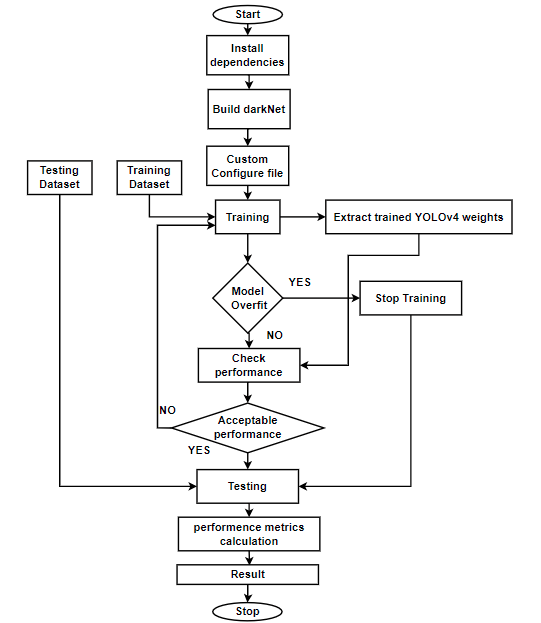
\includegraphics[scale=0.7]{50_Chapter_5/3.png}
    \caption{Working Flow}
    \label{Working Flow}
\end{figure}
Above figure shows the detailed flowchart of design and implementation from splitting dataset to evaluating result. All the necessary dependencies such as YOLOv4, CUDA, NumPy, and Python were installed from respective repositories. DarkNet [12] is a CUDA-based open-source neural network framework designed to support graphics processing units (GPU). A custom configuration file was created from the cloned YOLOv4 repository to build a custom object detector for tooth decay detection. All hyper parameters designed in the development of the custom object detector were detailed in the custom configuration file. The training module was then incorporated with a specific configuration file. Then, the model became ready to be trained with a custom dataset.\\
\textbf{Design Constraints and Parameters-Image Dataset}
\begin{enumerate}
    \item Number of Classes: 3
    \item Class name: Visible change without cavitation (0), Visible change with micro cavitation (1), Visible change with cavitation (2).
    \item Filter Size: 416*416
    \item Batch Size: 64
    \item Subdivision: 32
    \item Number of filters: (3+5)*3 = 24
\end{enumerate}
\textbf{Hyper parameters design}
\begin{enumerate}
    \item Image Size: 416*416
    \item Image channels: 3
    \item Kernel Size: 3*3
    \item Activation Function: Mish
    \item Batch Size: 64
    \item Max batches: 3*2000 = 6000
    \item Learning rate: 0.001
\end{enumerate}
The trainer's supervision was necessary for each epoch's parameter values, such as mAP, Accuracy, and Precision. To avoid model overfitting, training should be stopped after the given parameter values become constant or have very few changes. After the model was trained, best YOLOv4 weights are extracted which acts as a reference while testing the model on custom testing dataset. 
\section{YOLOv5 and Yolov6 Setup} A similar working flow as seen in fig 4.1 was used to train the dataset in YOLOv5 and YOLOv6 but without darknet. A dataset of 2618 photos was used to train YOLOv5 and Yolov6, with 86\% used for training, 9\% for validation, and 5\% for testing.
Both the model development started by installing necessary dependencies such as Python, Pytroch, YOLOv5, CUDA and roboflow from respective repositories. Datasets were uploaded and then exported into the YOLOv5 PyTorch format, which generated api keys for each dataset. It's worth mentioning that the Ultralytics solution requires a YAML file that defines where your training and test data should be stored. The Roboflow export also creates this format for us. 0 indicates visible changes without cavitation, 1 indicates visible changes with micro-cavitation, and 2 indicates visible changes with cavitation in the data.yaml file. Training configuration for YOLOv5 and YOLOv6:
\begin{table}[H]
\caption{YOLOv5 and YOLOv6 MODEL CONFIGURATIONS}
\centering
\begin{tabular}{|l|l|l|} 
\hline
\textcolor[rgb]{0.141,0.125,0.129}{Required Argument} & \textcolor[rgb]{0.141,0.125,0.129}{YOLOv5s} & \textcolor[rgb]{0.141,0.125,0.129}{YOLOv5m}  \\ 
\hline
\textcolor[rgb]{0.141,0.125,0.129}{Image Size}        & \textcolor[rgb]{0.141,0.125,0.129}{416x416} & \textcolor[rgb]{0.141,0.125,0.129}{416x416}  \\ 
\hline
\textcolor[rgb]{0.141,0.125,0.129}{Batch Size}        & \textcolor[rgb]{0.141,0.125,0.129}{16}      & \textcolor[rgb]{0.141,0.125,0.129}{32}       \\ 
\hline
\textcolor[rgb]{0.141,0.125,0.129}{Epoch}             & \textcolor[rgb]{0.141,0.125,0.129}{100}     & \textcolor[rgb]{0.141,0.125,0.129}{100}      \\
\hline
\end{tabular}
\end{table}
Training losses and performance data was saved to a log file created before with the —name flag when the model was trained. The weight values were saved in .pt files. On test photos, the best weights was applied and got somewhat improved accuracy in YOLOv5 and YOLOv6.
